\documentclass{article}
\usepackage[utf8]{inputenc}
\usepackage{graphicx}
\usepackage{subcaption}
\usepackage{amsmath}
\usepackage{setspace}
\usepackage[
  backend=biber,
  style=apa,
  citestyle=apa
]{biblatex}
\usepackage{geometry}
\geometry{
 a4paper,
 total={150mm,237mm},
 left=30mm,
 top=30mm,
 }

\renewcommand{\baselinestretch}{1.5} 
\addbibresource{references.bib}

\title{Bayesian Networks with Applications to Simulated Macroeconomic Timeseries}
\author{Emmet Hall-Hoffarth}
\date{June 2020}

\begin{document}

\maketitle

\section{Introduction}

DAGs \parencite{pearl2018book} are a non-parametric statistical technique for modelling causal probabilistic relationships. Under some conditions this and associated tools can allow for the inference of an interpretable structural model of a Data Generating Process (DGP) directly from some observed data. While there is much research still to be done regarding the theoretical properties of this methodology, the potential of automatically identifying causality already opens the door for numerous useful economic applications. To my knowledge, little work has been done in this area within the econometrics literature. In particular, Imbens (\citeyear{imbens2019potential}) notes a lack of concrete empirical examples demonstrating the usefulness of this methodology in the field of economics. Therefore, the purpose of this paper is to investigate one potential empirical application in the field of macroeconomics. 

The application involves modelling simulated data from well-known macroeconomic models. This application has a number of appealing properties. Firstly, because in a simulation the true DGP is known, it will be possible to precisely evaluate to what extent it is possible to identify the true underlying structure of the data using DAGs. Furthermore, in this controlled environment it is possible to ensure that the assumptions required by DAGs are satisfied, and therefore it provides a fair way to evaluate their applicability. Finally, these models are the central building blocks of modern macroeconomics and therefore provide a very relevant example of how DAGs can be applied in economics.

The remainder of this paper will be organised as follows. The second section will explain the fundamental elements of DAGs, with further discussion provided in an appendix. The third section will provide a review of the relevant literature in economics. The fourth section will discuss the empirical methodology employed in this paper. The fifth section will discuss the results that were obtained. The sixth section concludes.

\section{DAGs}

The fundamental assumption of a DAG is that the underlying DGP of some observed data can be represented as a Directed Acyclical Graph (DAG). Figure \ref{dag1} shows an example of a DAG. Each of the variables in the data forms a node in the graph, and these nodes are connected by arcs. The direction of each of the arcs represents the direction of causality in the sense of conditional probability. For example, if we observe the DAG $B \rightarrow A$, then A's distribution is conditional on B, whereas B's distribution is unconditional. In economic language the analogous interpretation is that B is exogenous while A is endogenous to or determined by B. As the name DAG implies, arcs are assumed to not create any cycles in the graph. This assumption is by no means innocuous, however, it is what gives DAGs the power to identify causal effects. For a given node, the set of nodes which have an arc pointing into that node are known as that node's parents, and the set of nodes that have an arc pointing into them from that node are known as that node's children. A root node is a node that has no arcs leading into itself, and a leaf node is a node that has not arcs leading out of itself.

\begin{figure}
  \centering
  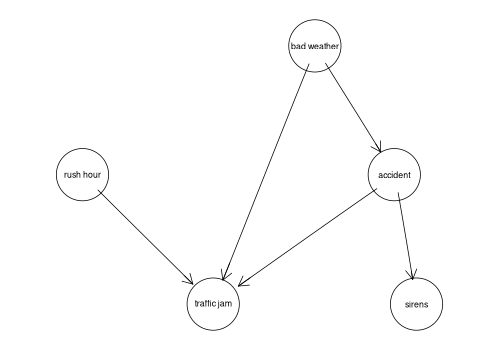
\includegraphics[width=0.8\textwidth]{images/trafficjam.png}
  \caption{An example of a simple DAG \parencite{traffic_jam}}
  \label{dag1}
\end{figure}

Each arc represents a conditional probability relationship. Nodes in the graph are assumed to be conditionally independent of all nodes which are not its parents. For example, in figure \ref{dag1}: 

\begin{equation}
  \label{eq1}
  p(sirens | data) = p(sirens | accident)
\end{equation}

These conditional probabilities are abstract in the sense that they could be treated as either discrete or continuous, and any distributional assumption of choice could be applied to them. While much of the literature surrounding DAGs focuses on the discrete case, in many economic applications continuous variables are the primary concern. This is possible as long as we are willing to make some distributional assumption about the nature of the conditional probability. The most common assumption here (and fortunately the most natural economic one), is that the conditional distributions follow a multivariate normal distribution of the conditioning variables. This is implies that conditional distributions are linear functions of conditioning variables with Gaussian errors, which is exactly the assumptions of simple, small-sample OLS regressions common in econometrics. Such models are sometimes known as "Gaussian DAGs." (GBN) For example:

\begin{equation}
  \label{eq2}
  sirens|data = sirens|accident = \alpha + \beta accident + \epsilon, \space \epsilon \sim N(0, \sigma^2)
\end{equation}

Therefore, this technique is "non-parametric" in the sense that we do not make any assumptions about which underlying relationships exist between variables (indeed, this is what we hope the model will tell us). However, we do make a distributional assumption about the conditional distributions.

When fully specified, a GBN consists of a system of linear equations that defines the joint distribution of the data. Because of the properties of the normal distribution, this means that we can express a GBN as a single joint normal distribution over the data, where the DAG specifies the exact restrictions that are imposed on the covariance matrix. In order to enhance clarity of exposition,in this paper all DAGs are assumed to be Gaussian unless otherwise specified. The primary benefit of this simplification is the fact that uncorrelatedness implies independence, although it is by no means necessary, and many of the same results hold for arbitrary distributional assumptions.

\subsection{Estimation and Identifiabiliy}

While the previous section outlined algorithms that can learn the structure of a graph it will be important to characterise the conditions under which this process can be expected to converge to a correct model of the underlying DGP. In other words, in order to believe that the DAG learned from some observed data is the correct model, what do we have to assume about the underlying DGP? Pearl (\citeyear{pearl2009causality}) defines a sufficient assumption as the "back-door criterion." A set of observed variables $z$ is said to satisfy the back-door criterion relative to $x$ and $y$ if:

\begin{enumerate}
  \item no node in $z$ is a decendent of $x$
  \item $z$ blocks every path between $x$ and $y$ that contains an arrow into $x$
\end{enumerate}

Here a path is any combination of arcs connecting one node to another (regardless of direction), and a path between $x$ and $y$ is blocked if $x$ and $y$ are independent in the DAG given $z$. Intuitively, this is the concept in economics commonly described as unconfoundedness. Although more general, it implies in particular that even if there are variables that are relevant to the true DGP that are unobserved, the DAG can still consistently estimate the causal effect of $x$ on $y$ as long as $x$ and $y$ have no common, unobserved causes (confounders). In particular, this identifying assumption allows for the causal effect of $x$ on $y$ to be observed, even if there is some unobserved variable $u$ that intermediates the causal path. This is profound in many economic applications where models assume that some unobservable function intermediates the relationships between observed variables. For example, a (unobservable) utility function intermediates the path between the observable determinants of demand such as price and preference ordering, and the quantity purchased. In this context, the front-door criterion implies that even if the true DGP contains a utility function which is unobservable to the model it is still possible correctly identify the causal effect of the demand determinants on the quantity purchased as long as all relevant determinants of the utility function are observed. The back-door criterion implies that complex functions that intermediate the relationship between observables are \textit{emergent} in the model without being explicitly assumed.

DAGs can also consistently identify a causal effect if it satisfies the "front-door criterion." A set of variables $z$ is said to satisfy the front-door criterion relative to variables $x$ and $y$ if it satisfies the following three assumptions \parencite{pearl2009causality}:

\begin{enumerate}
  \item $z$ blocks all directed paths from $x$ to $y$
  \item there are no unblocked back-door paths from $x$ to $z$
  \item all back-door paths from $z$ to $y$ are blocked by $x$
\end{enumerate}

\begin{figure}
  \centering
  \begin{subfigure}{0.45\textwidth}
    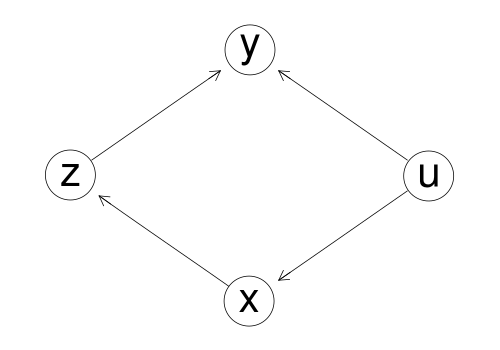
\includegraphics[width=\linewidth]{images/frontdoor.png} 
    \caption{Front-door criterion}
    \label{dag8_fd}
  \end{subfigure}
  %
  \begin{subfigure}{0.45\textwidth}
    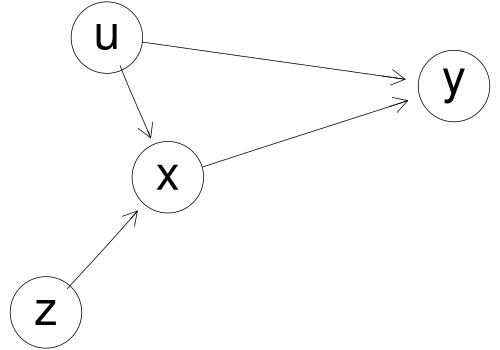
\includegraphics[width=\linewidth]{images/iv.png}
    \caption{Instrumental variables}
    \label{dag8_iv}
  \end{subfigure}
\end{figure}

The front-door criterion is demonstrated by figure \ref{dag8_fd}. Intuitively, what this allow s for is a sort of reverse instrumental variables identification where the instrument $z$ intermediates the causal path from $x$ to $y$ instead of being a parent/determinant of $x$. The assumptions here are similar in scope to those made in instrumental variables. The first assumption is akin to the exclusion restriction, the second exogeneity, and the third relevance.

Both the back-door and front-door criterion make strong assumptions about unobserved variables, which raises questions about their applicability. However, this problem is hardly specific to DAGs. Empirical economists are well acquainted with the difficulty of making arguments of unconfoundedness that are also required by many traditional econometric techniques, such as the exogeneity assumption required for instrumental variables. Because DAGs are an easily scalable machine learning technique they can add a sort of "brute force" tool to the empirical economics toolbox. This technique allows for causal inference by appeal to high-dimensional data sets rather than the clever arguments and insights usually required by econometric models over a small number of observed variables.

\subsection{Causality and Inference}

Now that the mathematical underpinnings of DAGs have been introduced, it will be necessary to discuss the concept of causality that they employ, because it is somewhat different from what we are used to in economics. Most modern empirical work in economics utilises the "Potental Outcome" causal framework \parencite{holland1986statistics}. In this framework a causal effect or treatment effect is defined as the difference between an outcome for an observational unit in the presence of a treatment $Y_i(1)$, and in the absence of the treatment $Y_i(0)$. This thinking is inspired by the medical and other physical sciences, where for example, the treatment effect of a medication on a patient's blood pressure is defined as the difference between the patient's blood pressure after taking the medication and \textit{what it would have been} if they had not taken the medication. Since in reality we can only ever observe one of these contingencies many statistical techniques have been developed that are able to consistently estimate this amount. Therefore, the potential outcomes framework can be said to make statements about counterfactuals, that is, the difference between outcomes in different states of the world.

The concept of causality that is relevant to DAGs is that of conditional independence. While this may seem unusual, this is actually akin to what is often assumed in macroeconomic theory, where every model has "exogenous shocks" that are the fundamental cause of the model dynamics. If we represent such macroeconomic models as DAGs these exogenous shocks would be the root nodes of the graph, because the root nodes of a DAG are assumed to be distributed independently of all other variables in the graph. In this framework the primary meaning of causality is exogeneity (that is in the literal sense, not being determined by what is observed), rather than treatment effects as in the potential outcomes framework. Since both of these concepts of causality (treatment effects and exogeneity) are commonly used in the field of economics one would like to believe that they are internally consistent, and indeed as I will argue in the remainder of this section, they are not incompatible. Indeed, DAGs are entirely consistent with potential outcomes and can be used to elicit counterfactuals / (average) treatment effects.

\begin{figure}
  \centering
  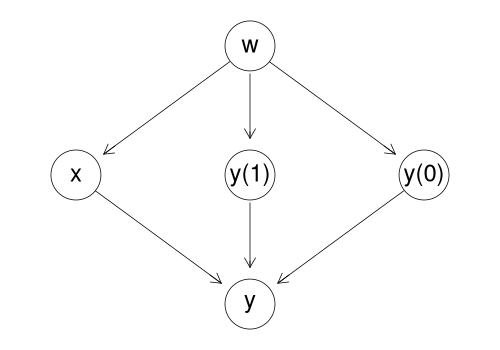
\includegraphics[width=0.8\textwidth]{images/potential_outcomes_dag.png}
  \caption{Potential Outcomes as a DAG}
  \label{dag6}
\end{figure}

Barr (\citeyear{barr2018causal}) gives an example of how the potential outcomes framework can be represented by a DAG, which is illustrated by figure \ref{dag6}. In this model, $w$ is a set of confounders, $x$ is the binary treatment of interest, $y(1)$ and $y(0)$ are the potential outcomes with and without the treatment respectively, and $y$ is $y(x)$. The fundamental assumption necessary for the consistent estimation of the average treatment effect here is that that given the confounders $w$ the treatment $x$ is independent of the potential outcomes. This is the assumption of unconfoundedness between the treatment and the treatment effects:
 
\begin{equation}
  x \perp \!\!\! \perp  (y(1), y(0)) | w
\end{equation}

In the graph, this assumption is illustrated by the fact that the only paths from $x$ to the potential outcomes are either through $y$, which is a collider which implies independence, or through $w$ which we have controlled for. This is an example of what Pearl (\citeyear{pearl2018book}) describes as the "back-door criterion" which he identifies as a necessary conditions for DAGs to have a causal interpretation. This illustrates the deep conceptual similarities between these frameworks.

Furthermore, DAGs can be used to estimate counterfactual outcomes, using what Pearl (\citeyear{pearl2014probabilistic}) describes as "do-calculus." This uses the notation $P(y|do(x=\bar{x}))$. The difference between this and $P(y|x=\bar{x})$ is that $do(x=\bar{x})$ reflects an exogenous change in $x$ to $\bar{x}$, whereas $P(y|x=\bar{x})$ suggests that the model is in a state that would predict that the variable $x$ takes on the value $\bar{x}$. Under some conditions, computing $P(y|do(x=\bar{x}))$ can achieved by breaking the links of $x$ with its parents and setting it to $\bar{x}$, and then observing $y$ in the model. This is demonstrated by Figure \ref{dag3}. For example, consider Figure \ref{dag3}. Suppose for simplicity that all of the variables are binary (1 in the presence of the event, 0 otherwise). On the LHS of the diagram we have the model for observed values of all of the variables. On the RHS we intervene on "accident." Notice that doing so breaks the link between "bad weather" and "accident." We can now estimate the causal treatment effect of an accident on the probability of a traffic jam given some values of "bad weather" and "rush hour" (in other words, all else equal) according to equation \ref{eq3}. This equation is very familiar, and is effectively the same as the calculation of an average treatment effect in the potential outcomes framework.

\begin{equation}
  \label{eq3}
  p(tj | bw = \bar{bw}, rh = \bar{rh}, do(a=1)) - p(tj | bw = \bar{bw}, rh = \bar{rh}, do(a=0))
\end{equation}

\begin{figure}

  \centering
  \begin{subfigure}{0.45\textwidth}
    \centering
    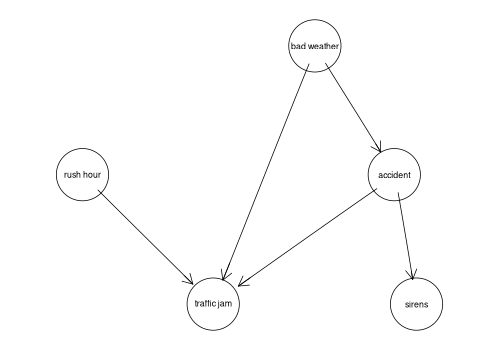
\includegraphics[width=\linewidth]{images/trafficjam.png} 
    \caption{No intervention}
  \end{subfigure}
  %
  \begin{subfigure}{0.05\textwidth}
    \centering
    $\rightarrow$
  \end{subfigure}
  %
  \begin{subfigure}{0.45\textwidth}
    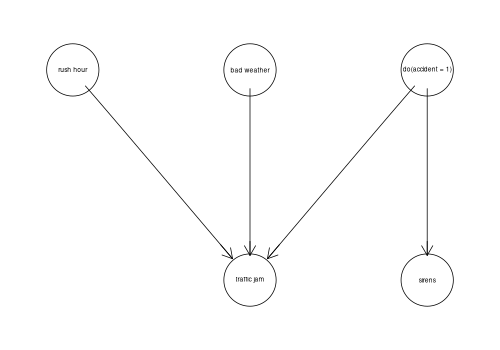
\includegraphics[width=\linewidth]{images/trafficjam_intervention.png}
    \caption{Intervention}
  \end{subfigure}

  \caption{An example of intervention}
  \label{dag3}
\end{figure}

In addition, there are other kinds of possible prediction exercises that we may be interested in with some economic interpretation. Since the model defines every endogenous variable as a (linear) function of the exogenous shocks it can be interpreted as a structural model of the data. Therefore, we might compute impulse response functions (IRFs) for each endogenous variable in the model to one or more shocks.

\subsection{Limitations}

Before continuing I will point out some of the limitations both of this methodology, and of my own knowledge in order to give some idea of the pitfalls that needed to be taken into account in the course of carrying out this research.

\subsubsection{Simultaneity}

The concept of a DAG, while a powerful tool, is not a perfect model for all data. The strongest assumption is that it is directed. In many economic applications, while we may believe that some variables are truly exogenous such that they must be causes of movement in endogenous variables and not the other way around, we usually also assume that some or all of the endogenous variables are determined in general equilibrium, that is to say there is not necessarily a directionality to every relationship between endogenous variables. The problem of simultaneity is important, but there are ways which we can work with it in the DAG framework. I will propose two solutions to this problem: the first is that many relationships that we commonly think of as simultaneous have a mathematically equivalent fully directed model, and the second is that it is possible to relax the assumption that the graph is fully directed.

\begin{figure}

  \centering
  \begin{subfigure}{0.45\textwidth}
    \centering
    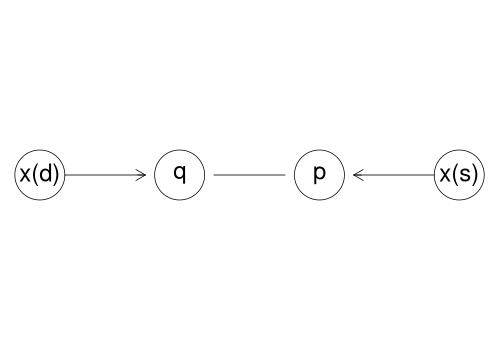
\includegraphics[width=\linewidth]{images/simultaneous.png} 
    \caption{Explcit simultaneity}
    \label{dag7_a}
  \end{subfigure}
  %
  \begin{subfigure}{0.05\textwidth}
    \centering
    $\iff$
  \end{subfigure}
  %
  \begin{subfigure}{0.45\textwidth}
    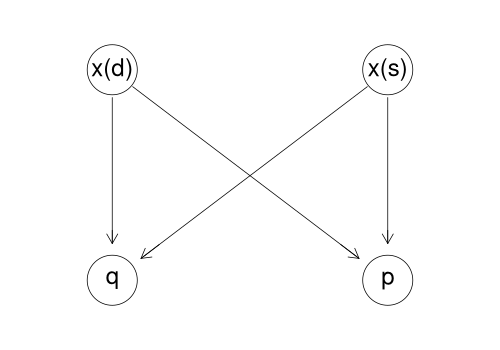
\includegraphics[width=\linewidth]{images/directed.png}
    \caption{Directed simultaneity}
    \label{dag7_b}
  \end{subfigure}

  \caption{An example of directing simultaneity}
  \label{dag7}
\end{figure}

In order to see why explicitly modelling simultaneity may not be necessary, consider figure \ref{dag7}, which is inspired by \citeauthor{imbens2019potential} (\citeyear{imbens2019potential}). Figure \ref{dag7_a} shows a simple model of supply and demand where quantity $q$ and price $p$ are determined simultaneously in the presence of demand shock $x(d)$ and supply shock $x(s)$. The relationship between quantity and price is simultaneous because changes in each one affect the other. However, the relationships implied by figure \ref{dag7_a} can just as well be represented by the fully directed graph in figure \ref{dag7_b}. To see this consider the following equations which are implied by figure \ref{dag7_a}:

\begin{equation}
  p = \alpha_p + \beta_{ps} x(s) + \beta_{pq} q + \epsilon_{p}
\end{equation}
\begin{equation}
  q = \alpha_q + \beta_{qd} x(d) + \beta_{qp} p + \epsilon_{q}
\end{equation}

By substituting $p$ into the equation for $q$ and vice versa it can be shown that this system of equations is equivalent to:

\begin{equation}
  \label{price_eq}
  p = \frac{1}{1-\beta_{pq}\beta_{qp}}[(\alpha_p + \beta_{pq} \alpha_q) + \beta_{ps} x(s) + \beta_{pq} \beta_{qd} x(d) + (\epsilon_p + \beta_{pq} \epsilon_q)]
\end{equation}
\begin{equation}
  \label{quantity_eq}
  q = \frac{1}{1-\beta_{qp}\beta_{pq}}[(\alpha_q + \beta_{qp} \alpha_p) + \beta_{qd} x(d) + \beta_{qp} \beta_{ps} x(s) + (\epsilon_q + \beta_{qp} \epsilon_p)]
\end{equation}

Which is (a version of) what is represented by figure \ref{dag7_b}. At this point I will note the relevance of the Lucas (\citeyear{lucas1976econometric}) critique. The model in \ref{dag7_b} is a reduced form estimation of the model in \ref{dag7_a}, and as such, it will be impossible to identify the policy parameters $\beta_{pq}$ and $\beta_{qp}$. In general, DAGs are a statistical technique that rely only on observed data, and therefore, they will not be immune to the Lucas critique. However, we \textit{can} identify the impact of exogenous shocks to the model. In the context of this example, this means that while the DAG cannot consistently estimate the supply and demand elasticities, it can consistently estimate the effect of a demand shock $x(d)$ or supply shock $x(s)$ on the equilibrium of the model. In the context of macroeconomic models we are often interested in computing IRFs which is the equilibrium effect of an exogenous shock to the model. This argument illustrates why even though we believe that many of the variables in these macroeconomic models are simultaneously determined, we can still estimate IRFs using DAGs. More generally, although DAGs might not be able to identify all structural parameters that economists might be interested in, they are nonetheless able to identify causal effects and in many applications this is likely sufficient. For this reason, the discussion in the applications in this paper will focus on identifying the root nodes of a graph and their effects, while less emphasis will be placed on the relationships further down the causal tree.

However, it is also possible to explicitly model simultaneity in the context of graphical models. As discussed earlier, constraint based structure learning algorithms do not force a direction onto every arc, so it is entirely possible for sturcure learning to result in a Partially Directed Acyclical Graph (PDAG). Such models are known as hybrid networks or chain graphs, originally proposed by Wermuth and Lauritzen (\citeyear{wermuth1990substantive}). Recall that the DAG assumption can be characterised as a set of constraints on the covariance matrix of the joint normal distribution. In a hybrid network then there are no constraints on the partition of the covaraince matrix for the variables in the model that are assumed to be simultaneous. Note however, that while this approach may be more comfortable from the economic point of view it will still not immunise the model to the Lucas critique. Unfortunately, I was unable to find any convincing implementations which allow for hybrid networks. Therefore, all of the graphs that I use in my application are fully directed and used with appeal to the previous argument.

\section{Liturature Review}

\section{Methodology}

\subsection{Estimation}

There are two fundamental problems to solve when estimating a DAG. The first is known as "parameter learning," and the other "structure learning." Given a DAG as in Figure \ref{dag1}, the first task is simply to estimate the parameters of the network, such as $\alpha$ and $\beta$ in Equation \ref{eq2}. This is usually done via maximum likelihood, however, other "score" functions are available such as the Bayesian Information Criterion (BIC) \parencite{chen1998speaker}.

\begin{figure}
  \centering
  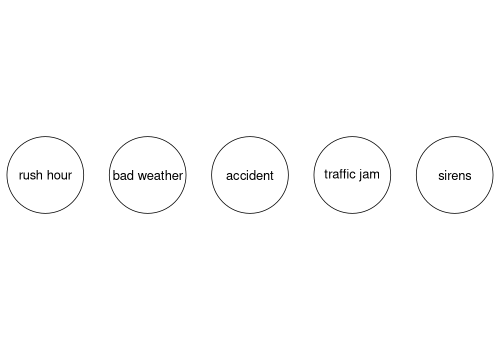
\includegraphics[width=0.8\textwidth]{images/trafficjam_unfit.png}
  \caption{A DAG before structure learning}
  \label{dag2}
\end{figure}

The second task, as demonstrated by Figure \ref{dag2} is that if we just start with some data it is not obvious which conditional probabilities to estimate in the first place. One way of achieving this is for the researcher to specify explicitly which conditional probabilities should be present in the graph, and simply fit the parameters of that graph. This however, is not what I am particularly interested in. If this is done the researcher has effectively specified a system of linear regressions to be estimated, probably based on some economic model that they already had in mind, and while this is then automatically encapsulated in a convenient, easily interpreted representation of the underlying assumptions, it seems nothing of profound economic significance is achieved in this case. 

A more more exciting approach is to algorithmically learn the structure of the graph, that is to learn a structural model, directly from observed data. One "brute force" method to solving this problem is to compute the posterior likelihood of every possible network, however, this number is super-exponential in the number of variables such that it becomes very computationally expensive, very quickly \parencite{chickering1996learning}. As a response to this, many heuristic approximation techniques have been developed. These can be grouped into two categories: constraint-based and score-based structure learning algorithms \parencite{spirtes1991algorithm} \parencite{verma1991equivalence}. 

\begin{figure}

  \centering
  \begin{subfigure}{0.3\textwidth}
    \centering
    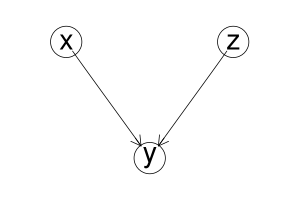
\includegraphics[width=\linewidth]{images/collider.png} 
    \small
    \begin{equation*}
      x = \epsilon_{x}
    \end{equation*}
    \begin{equation*}
      y = \alpha_y + \beta_{yx} x + \beta_{yz} z + \epsilon_{y}
    \end{equation*}
    \begin{equation*}
      z = \epsilon_{z}
    \end{equation*}
    \caption{Collider}
    \label{collider}
  \end{subfigure}
  %
  \begin{subfigure}{0.3\textwidth}
    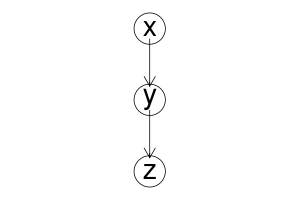
\includegraphics[width=\linewidth]{images/chain.png}
    \small
    \begin{equation*}
      x = \epsilon_{x}
    \end{equation*}
    \begin{equation*}
      y = \alpha_y + \beta_{yx} x + \epsilon_{y}
    \end{equation*}
    \begin{equation*}
      z = \alpha_z + \beta_{zy} y + \epsilon_{z}
    \end{equation*}
    \caption{Chain}
    \label{chain}
  \end{subfigure}
  %
  \begin{subfigure}{0.3\textwidth}
    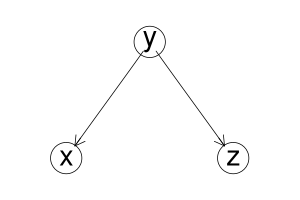
\includegraphics[width=\linewidth]{images/fork.png}
    \small
    \begin{equation*}
      x = \alpha_x + \beta_{xy} y + \epsilon_{x}
    \end{equation*}
    \begin{equation*}
      y = \epsilon_{y}
    \end{equation*}
    \begin{equation*}
      z = \alpha_z + \beta_{zy} y + \epsilon_{z}
    \end{equation*}
    \caption{Fork}
    \label{fork}
  \end{subfigure}

  \caption{The three possible v-structures of a 3 node DAG. Error terms $\epsilon$ are all i.i.d. Gaussian shocks.}
  \label{dag5}
\end{figure}

Constraint-based algorithms rely on the fact that changing the direction of an arc changes the conditional independences implied by the graph, the presence of which can be tested for in the data. To see how the DAG assumptions can be sufficient to learn a causal model in this way, consider the example in figure \ref{dag5}. Suppose we have a graph with three nodes, such that no one node is completely independent from the other two (as this would make the graph trivial, and we could in any case rule out this case with an independence test). Furthermore, the graph cannot have all three possible arcs because it would either contain a cycle, or the third arc would imply a relationship which is redundant given the other two. Then the graph must have exactly two arcs. Given this, there are exactly three possible permutations of the network, which are the three shown in figure \ref{dag5}. These are known as the the three canonical "v-structures." \parencite{pearl2014probabilistic} These structures are partially identifiable from observational data because they imply different testable hypotheses about conditional independence. While the chain and fork imply that x and z are unconditionally dependent and only independent conditional on y, the collider implies exactly the opposite; that x and z are unconditionally independent and dependent conditional on y. Given some observed data we can easily test for the presence of conditional and unconditional independence using a $\chi^2$ test. The results of these tests can be used to rule out certain network structures which would be inconsistent with the observed data. Although for every set of three variables the network is only partially identifiable, full identification can (but will not always) be achieved when more variables are observed, by comparing overlapping triplets of variables and progressively reducing the set of network structures that are consistent both with the DAG assumptions and with the observed conditional independences.

Score-based methods as the name implies assign some score to every network based on its predictive accuracy and then use gradient-decent to identify the optimum network structure. There are a number of scoring functions and hill climbing algorithms that one can use to achieve this. 

The major benefit of the constraint based method is that it directly utilises conditional independence as a primitive, which is the concept of causality that DAGs seek to identify. This is in contrast to score base methods, which effectively maximise the predictive accuracy of the model, and there is seemingly no guarantee that the most predictive model is the most likely causal explanation. The major benefit of score based methods on the other hand is that they will always converge to a single fully directed graph as a solution whereas constraint based methods, because V-structures are only partially identifiable, may not be able to identify a unique solution. Instead, when the graph is only partially identifiable, the algorithm will return an undirected graph, because that arc could take on face either direction and the graph would still be consistent with both the DAG assumption and the observed conditional independences. By permuting the two possible directions of each undirected arc we arrive at a set of graphs that are said to be "observationally equivalent." This is problematic because it is difficult or impossible to fit parameters to graphs that are not fully directed (see limitations section).  

Fortunately, these two methods can be combined into so called "hybrid" structure learning methods which use the strengths of both methods to counter the weaknesses of the other \parencite{scutari2014multiple} \parencite{friedman2013learning}. In this method the algorithm maximises a score function, but the number of parents that each node can have is restricted. The main benefit of this is a large gain computation efficiency because the search space is dramatically reduced, and theoretically it has the benefits of both constraint based and score based learning. However, while resulting the graph is always directed, it does not always correctly reflect the observed v-structures because it trades off constraint satisfaction and score maximisation.

I believe that structure learning is the greatest contribution of the DAG framework. Many of the topics in this paper should seem quite familiar to any econometrician because they are fundamentally the same as some basic econometric concepts, although perhaps expressed through different language. However, the novel benefit of using this method is that we are effectively able to estimate a structural model directly from the data, without first having to specify which relationships we believe should be present. This is a very powerful concept because it removes researcher bias by allowing the data to speak for itself.

For the application in this paper I have used the "bnlearn" package \parencite{scutari2010bnlearn} for R. I used the provided hybrid structure learning algorithm, rsmax2 with the pc.stable structure restriction algorithm and the log likelihood score function. The parameters of the model are then fit via maximum likelihood. 

\subsection{Dynamics} \label{dynamics}

When analysing macroeconomic data it is essential to consider any dynamic interactions that are present. In the discrete case (which is the relevant case for economic applications) these interactions can be captured in a straightforward manner by including the lags of some/all model variables as nodes in the DAG. Such models are sometimes called dynamic Bayesian networks \cite{ghahramani1997learning}. The important modelling decision that must be made is which variables to include lags for and how many lags to include. In particular, this may be difficult in the machine learning context where little can be assumed of variables ex-ante. Therefore, this section will discuss an agnostic approach to dynamic modelling of DSGE data using DAGs.

DSGE models contain both "control" variables which are determined independently across time in each period, and "state" variables who's value depends on the past. In general state variables may depend on values arbitrarily far into the past, however, most DSGE models, including all of those which are simulated in this paper have the Markov property, that is, conditional on the previous period, values in the current period are independent of values in all earlier periods.Therefore, when lags are included for variables it is only necessary to include the first lag. By definition, only state variables depend on the past of the model, so the ground-truth DAG for a DSGE model would only include lags for state variables. However, in the observational context it may be difficult to determine which variables are in fact the state variables of the ground-truth model because control variables may demonstrate a high degree of auto-correlation. The solution employed in this paper is simply to include the first lags of all variables. However, in order to avoid spurious connections in the resulting DAG a blacklist is implemented such that any lags which are connect to the rest of the DAG must be root nodes. This is justified because the DAG does not allow for simultaneity, so the past values of any variable must be exogenous relative to the current ones, even those which are determined by rational expectations. 

\section{Data}

In order to demonstrate the capability of the DAG methodology empirically I have chosen to use simulated data from macroeconomic models. There are a few key reasons why I have chosen to work with this data. Firstly, since the model that simulates the data is known it is possible to evaluate whether the structure learning has succeeded in identifying the underlying relationships in the data. In other words, since the true DGP is known it is possible to infer whether the estimated DAG correctly represents the underlying DGP. Secondly, in the context of a log-linearized macroeconomic model the distributional assumption that conditional distributions are linear with Gaussian errors, and structural assumption that the DGP is a DAG are in fact correct. Finally, since these models are central to modern macroeconomics it provides an excellent opportunity to demonstrate the applicability of DAGs in economic applications.

In order to collect simulated data I consulted a github repository containing Dynare code to replicate a number of well known macroeconomic models \parencite{pfeifer2020}. In particular, I chose to model the baseline RBC model as a simple case and the \citeauthor{smets2007shocks} (\citeyear{smets2007shocks}) model for a more difficult and complex modelling challenge. I modified the simulation code slightly such that rather than impulse response functions the output of the simulation would be a file containing (n) observations of i.i.d. draws of the exogenous shocks, and the associated observed values of the other variables in the model. This file was then used as the input for fitting DAGs.

\section{Results}

\subsection{RBC}

\subsubsection{Model}

\begin{table}
  \centering
  \begin{tabular}{|l|l|l|}
    \hline
    Symbol & Name & Type \\
    \hline
    $eps\_g$ & government spending shock & shock \\
    $eps\_z$ & technology shock & shock \\
    $g$ & government spending level & state \\
    $z$ & technology process level & state \\
    $k$ & capital & state \\
    $w$ & wage rate & control \\
    $r$ & return to capital & control \\
    $y$ & output & control \\
    $c$ & consumption & control \\
    $l$ & hours worked & control \\
    $i$ & investment & control \\ \cline{2-2}
    \hline
  \end{tabular}
  \caption{Description of Variables}
  \label{tab1}
\end{table}

The first model which I have chosen to evaluate is a the baseline RBC model provided by \citeauthor{pfeifer2020} (\citeyear{pfeifer2020}). This model includes 11 variables which are summarized by Table \ref{tab1}. Using the default specification a sample of 10000 observations was generated. 

\subsubsection{Structure Learning}

\begin{figure}
  \centering
  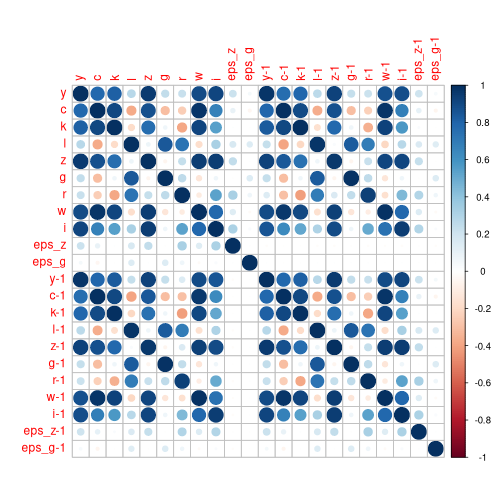
\includegraphics[width=0.8\linewidth]{images/rbc_correlation.png}
  \caption{Correlation matrix of baseline RBC model}
  \label{rbccorr}
\end{figure}

\begin{figure}

  \centering
  \begin{subfigure}{0.6\textwidth}
    \centering
    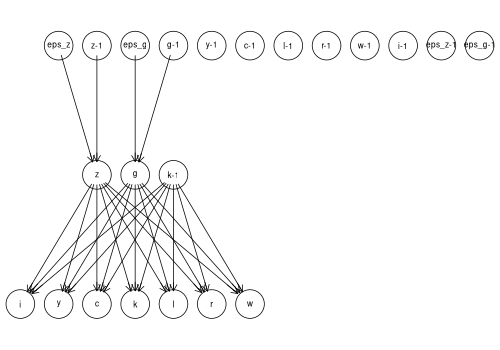
\includegraphics[width=\linewidth]{images/rbc_true_dag.png} 
    \caption{Ground Truth DAG}
    \label{gtdag}
  \end{subfigure}
  %
  \begin{subfigure}{0.6\textwidth}
    \centering  
    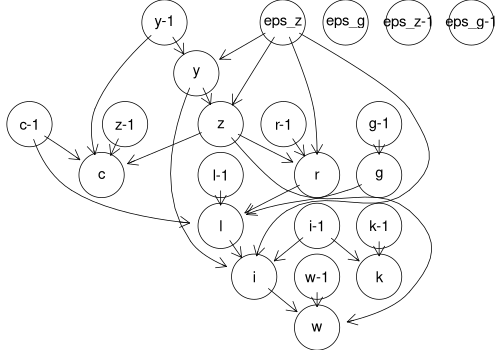
\includegraphics[width=\linewidth]{images/rbc_hybrid_dag.png}
    \caption{Hybrid DAG}
    \label{hdag}
  \end{subfigure}

  \caption{Structure of DAGs manually and algorithmically fit to RBC model data.}
  \label{rbcdags}
\end{figure}

Figure \ref{rbcdags} shows the ground truth DAG, as well as a DAG learned using the hybrid structure learning algorithm. There are a few results to note here. Firstly, the root nodes of the learned graph are not completely correct. While the technology shock and the lagged state variables are correctly identified as root nodes, the lags of various control variables are also identified as root nodes, whereas in the ground truth model these are independent of the DAG. This is because, as demonstrated by Figure \ref{rbccorr} we observe very high autocorrelation for every variable in the model. However, this will turn out to not be very problematic when we consider the IRFs from this DAG. Also it is notable that $eps\_g$ is not connected to the rest of the graph. This is because in the default specification the autocorrelation parameter for $g$ is very close to 1 (0.989), resulting in very low parial correlation between $g$ and $eps\_g$ \footnote{Attempting this calculation results in a matrix inversion error because $g$ and $g_{t-1}$ are so colinear.}.

\subsubsection{IRFs}

\begin{figure}

  \centering
  \begin{subfigure}{0.8\textwidth}
    \centering
    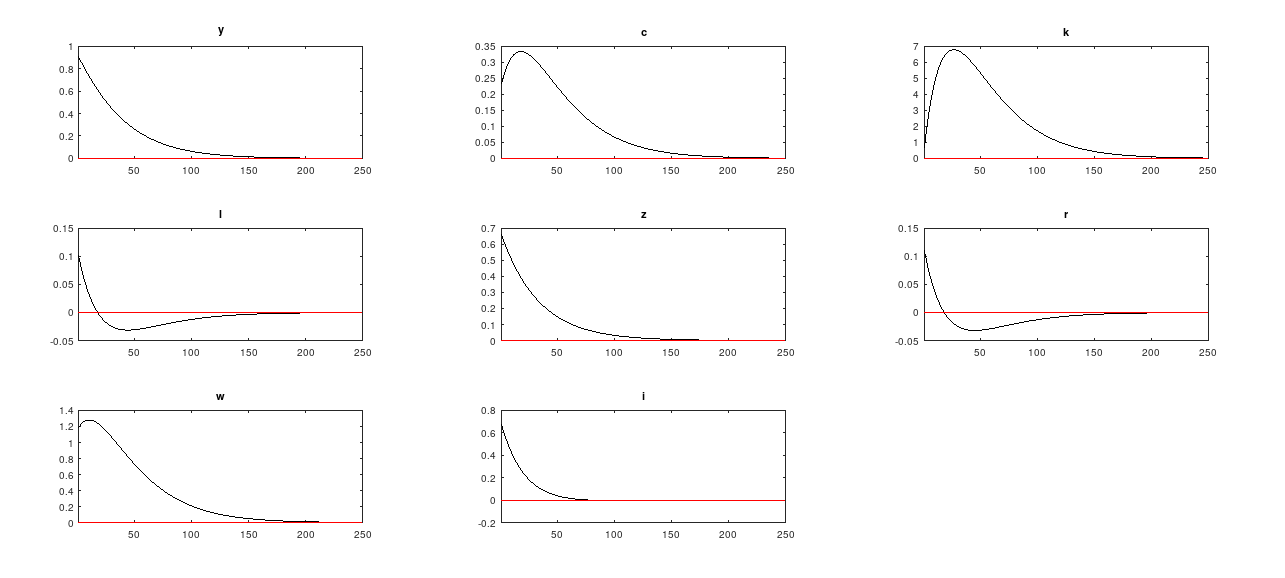
\includegraphics[width=\linewidth]{images/rbc_sim_irf.png} 
    \caption{Original Simulation}
    \label{simirf}
  \end{subfigure}
  %
  \begin{subfigure}{0.8\textwidth}
    \centering  
    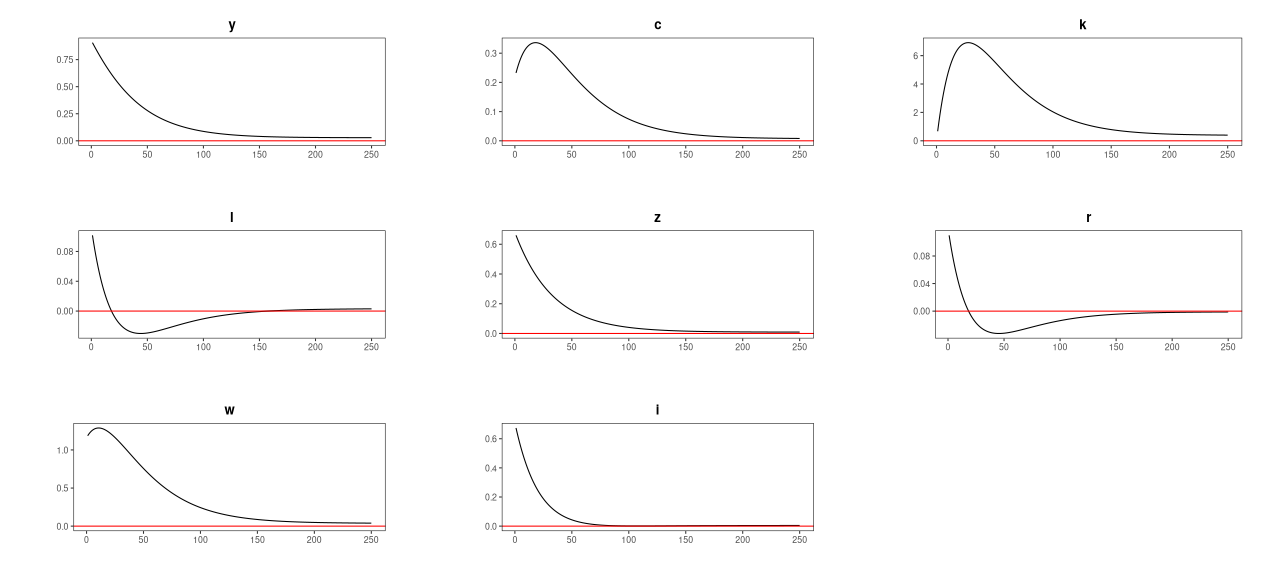
\includegraphics[width=\linewidth]{images/rbc_true_dag_irfs.png}
    \caption{Ground Truth DAG}
    \label{gtirf}
  \end{subfigure}
  %
  \begin{subfigure}{0.8\textwidth}
    \centering  
    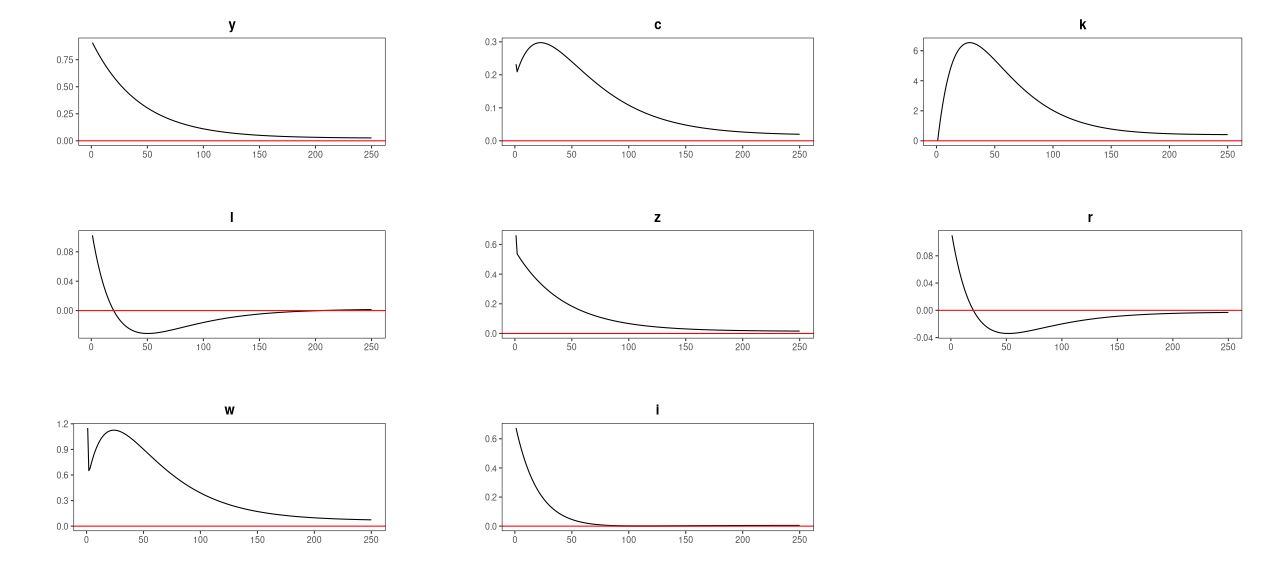
\includegraphics[width=\linewidth]{images/rbc_hybrid_dag_irfs.png}
    \caption{Hybrid DAG}
    \label{hirf}
  \end{subfigure}

  \caption{IRFs generated by the original model and various DAGs generated on the simulated data.}
  \label{dag10}
\end{figure}

Figure \ref{dag10} illustrates the IRFs to a technology shock of 1 standard deviation for the original simulation (\ref{simirf}) in comparison with those generated by various DAGs. The ground truth DAG replicates the oringal simulations' IRFs almost perfectly, as it should since all of the necessary assumptions are satisfied, and by constructi this DAG specifies the same linear system of equations as the solution to the simulated model. More notable however, is that the structure learned using the hybrid structure learning method also produces very accurate IRFs, despite the fact that it does not have all of the correct root nodes. The only discrepancy seems to be a small jump in the first period for $c$, $z$, and $w$. This demonstrates that the algorithm has nonetheless converged to a genuine causal model of the data.

\subsection{Smets and Wouters (2007)}

\begin{figure}

    \centering
    \begin{subfigure}{0.3\textwidth}
      \centering
      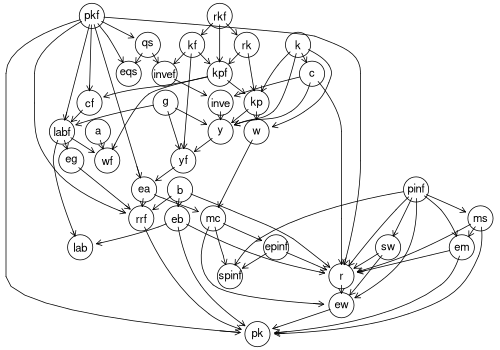
\includegraphics[width=\linewidth]{images/sw_init.png} 
      \caption{Unconstrained}
      \label{init}
    \end{subfigure}
    %
    \begin{subfigure}{0.3\textwidth}
      \centering  
      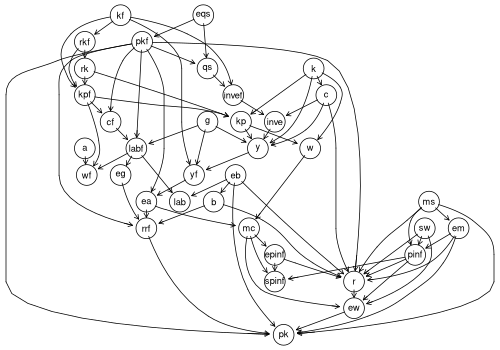
\includegraphics[width=\linewidth]{images/sw_equiv.png}
      \caption{Observationally Equivalent}
      \label{equiv}
    \end{subfigure}
    %
    \begin{subfigure}{0.3\textwidth}
      \centering  
      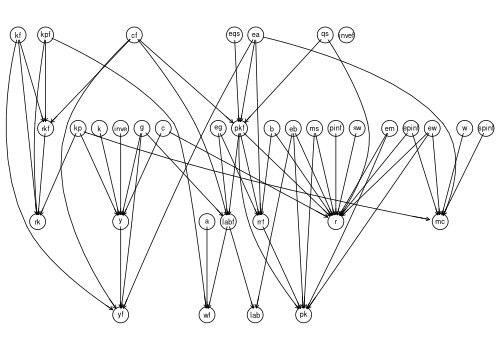
\includegraphics[width=\linewidth]{images/sw_bl.png}
      \caption{Forced Exogenous Roots}
      \label{bl}
    \end{subfigure}
  
    \caption{Three different approaches to structure learning with the Smets and Wouters model.}
    \label{dag9}
  \end{figure}

\subsubsection{Model}

This model from this seminal paper is quite complex and contains a large number of variables and thus it provides difficult challenge with which to demonstrate the capabilities of the DAG methodology. 

This model contains seven exogenous shocks: a productivity shock (ea), a risk premium shock (eb), a government expendiature shock (eg), an investment specific technology shock (eqs), a monetary policy shock (em), a price markup shock (epinf), and a wage markup shock (ew). Furthermore, these shocks all contribute to the AR/MA process of the stock of technology (a), risk premium (b), government spending (g), investment specific technology (qs), and, money supply (ms), price shock (spinf), and wage shock (sw), all of which are exogenous from a cross sectional perspective. The model contains a number of state variables \footnote{As the state variables of the model are never explicitly stated in the original paper, I take them to be the set of all variables whose value is a function of its own lagged value in the linear model.} that are exogenous from the cross sectional perspective: flexible economy capital services (kf), capital stock (kpf), investment (invef), consumption (cf), as well as nominal rigidity economy capital services (k), capital (kp), investment (inve), consumption (c), inflation (pinf), and, wages (w). Taken together the model contains 24 variables that are exogenous from the cross sectional perspective.

\subsubsection{Structure Learning}

We now consider the extent to which DAG structure learning is able to identify these exogenous variables. Before beginning some light data cleaning was performed. Difference variables were removed because they contain information about the past, as for now, we wish to consider cross-sectional behavior. Finally, "observed" values were dropped as these are redundant. After these simplifications 36 variables remained in the data, for which 10000 observations were made available. Figure \ref{init} shows the result of performing the hybrid structure learning algorithm on this data. This graph has 7 root nodes: rkf, pkf, k, pinf, a, b, and, g, 5 of which are in fact exogenous. The two endogenous variables that are identified as root nodes are rkf and pkf. This result is not optimal, however, there are some tricks we can use to arrive at a more sensible model.

One simple way to improve the model is to consider the class of observationally equivalent models which can be achieved by changing the direction of some arcs in such a way that the resulting graph is still consistent with the observed v-structures. For example we can reverse the arc $b \rightarrow eb$ because clearly the causality runs the other way around. Making all of the possible corrections we arrive at figure \ref{equiv}. The root nodes of this graph are kf, k, a, g, ms, sw, eb, eqs, all of which are in fact exogenous. This is a much better result in the sense that it achieves no "false-positives" for exogeneity, however, it does not identify all exogenous variables. Intuitively, this is possible because there are variables in the model which are nearly colinear with the exogenous shocks (for example the correlation between eb and b is 0.99, because preference shocks demonstrate very little time series behavior in the calibration of the model). If this is the case then the variables effectively measure the same quantity, and thus lack inherent causality, so the choice of arc direction between them is essentially arbitrary. Therefore, when using DAGs one should be weary of colinearity in the observed data. Through some experimentation I have found that selectively excluding variables that appear to be colienar with another can greatly improve the structure learning results, however, I have excluded these results until I can implement this feature selection in a systematic way.

Figure \ref{bl} shows a stucture that was learned after implementing a blacklist that prevents any of the exogenous variables from having parents, effectively guaranteeing that the set of root nodes will be exactly the set of exogenous variables in the model. Since this is rather trivial with simulated data the purpose of including this model is to provide a benchmark to evaluate the performance of the algorithmically developed structures.

\subsubsection{Evaluation}

\section{Conclusion}

\printbibliography

\end{document}
